\subsection{Weakly Non-linear Modal DBI Reduction}
  \label{subsec:weakly-nonlinear-dbi-reduction}

  To incorporate the first Born--Infeld correction, consider the discrete DBI Lagrangian
  \begin{equation}
    \label{eq:dbi-lagrangian}
    L
    =
    -c_\chi^2 \sum_v \sqrt{1 - \dot{\chi}_v^2/c_\chi^2}
    - \tfrac{1}{2} \sum_{v,w} \chi_v \mathcal{L}_{vw} \chi_w.
  \end{equation}
  For a single eigenmode,
  \begin{equation}
    \chi_v(t) = q(t)\psi_n(v),
  \end{equation}
  with $\mathcal{L}\psi_n = \lambda_n \psi_n$ and $\|\psi_n\|_2 = 1$, this reduces to
  the exact one-mode Lagrangian
  \begin{equation}
    \label{eq:exact-mode-lagrangian}
    L_n[q]
    =
    -c_\chi^2 \sum_v \sqrt{1 - \psi_n(v)^2 \dot{q}^{\,2}/c_\chi^2}
    - \tfrac{1}{2}\lambda_n q^2.
  \end{equation}

  Expanding the square root for $|\dot{q}| \ll c_\chi$ gives
  \begin{equation}
    \label{eq:mode-lagrangian-expansion}
    L_n[q]
    =
    \mathrm{const}
    + \tfrac{1}{2}\dot{q}^{\,2}
    + \frac{\kappa_n}{8c_\chi^2}\dot{q}^{\,4}
    - \tfrac{1}{2}\lambda_n q^2
    + \mathcal{O}(c_\chi^{-4}),
  \end{equation}
  where
  \begin{equation}
    \label{eq:kappa-def}
    \kappa_n := \sum_v \psi_n(v)^4.
  \end{equation}
  The corresponding Euler--Lagrange equation is
  \begin{equation}
    \label{eq:weakly-nonlinear-mode-equation}
    \left(
      1 + \frac{3\kappa_n}{2c_\chi^2}\dot{q}^{\,2}
    \right)\ddot{q}
    + \lambda_n q
    = 0.
  \end{equation}

  Using the harmonic-balance ansatz
  \begin{equation}
    q(t) \approx a_n \cos(\omega_n t),
  \end{equation}
  and keeping only the fundamental harmonic, one obtains the first
  amplitude-dependent correction
  \begin{equation}
    \label{eq:omega-shift-square}
    \omega_n^2(a_n)
    \approx
    \lambda_n
    \left(
      1 - \frac{3\kappa_n\lambda_n a_n^2}{8c_\chi^2}
    \right),
  \end{equation}
  or equivalently
  \begin{equation}
    \label{eq:omega-shift}
    \omega_n(a_n)
    \approx
    \sqrt{\lambda_n}
    \left(
      1 - \frac{3\kappa_n\lambda_n a_n^2}{16c_\chi^2}
    \right).
  \end{equation}
  The DBI correction is therefore a softening non-linearity.

  In the canonical $Q_8$ basis, the quartic shape factor is explicit.
  For the one-dimensional nontrivial abelian sectors,
  \begin{equation}
    \label{eq:kappa-abelian}
    \kappa_{\rho_k}
    =
    \sum_{v \in Q_8} \left(\frac{1}{\sqrt{8}}\right)^4
    =
    \frac{1}{8},
    \qquad
    k = 1,2,3.
  \end{equation}
  For each canonical basis vector in the $\rho_4$ sector,
  \begin{equation}
    \label{eq:kappa-nonabelian}
    \kappa_{\rho_4}
    =
    4 \left(\frac{1}{2}\right)^4
    =
    \frac{1}{4}.
  \end{equation}

  However, rewriting the correction in terms of the effective amplitude
  $A_n = a_n\|\psi_n\|_\infty$ gives
  \begin{equation}
    \label{eq:omega-shift-effective}
    \omega_n^2(A_n)
    \approx
    \lambda_n
    \left(
      1
      - \frac{3\lambda_n A_n^2}{8c_\chi^2}
      \frac{\kappa_n}{\|\psi_n\|_\infty^2}
    \right).
  \end{equation}
  In the canonical $Q_8$ basis,
  \begin{equation}
    \frac{\kappa_{\rho_k}}{\|\psi_{\rho_k}\|_\infty^2}
    =
    \frac{(1/8)}{(1/\sqrt{8})^2}
    =
    1,
    \qquad
    \frac{\kappa_{\rho_4}}{\|\psi_{\rho_4}\|_\infty^2}
    =
    \frac{(1/4)}{(1/2)^2}
    =
    1.
  \end{equation}
  Therefore
  \begin{equation}
    \label{eq:omega-shift-effective-q8}
    \omega_n^2(A_n)
    \approx
    \lambda_n
    \left(
      1 - \frac{3\lambda_n A_n^2}{8c_\chi^2}
    \right)
  \end{equation}
  in both the nontrivial abelian and non-abelian sectors.

  \begin{figure}[t]
    \centering
    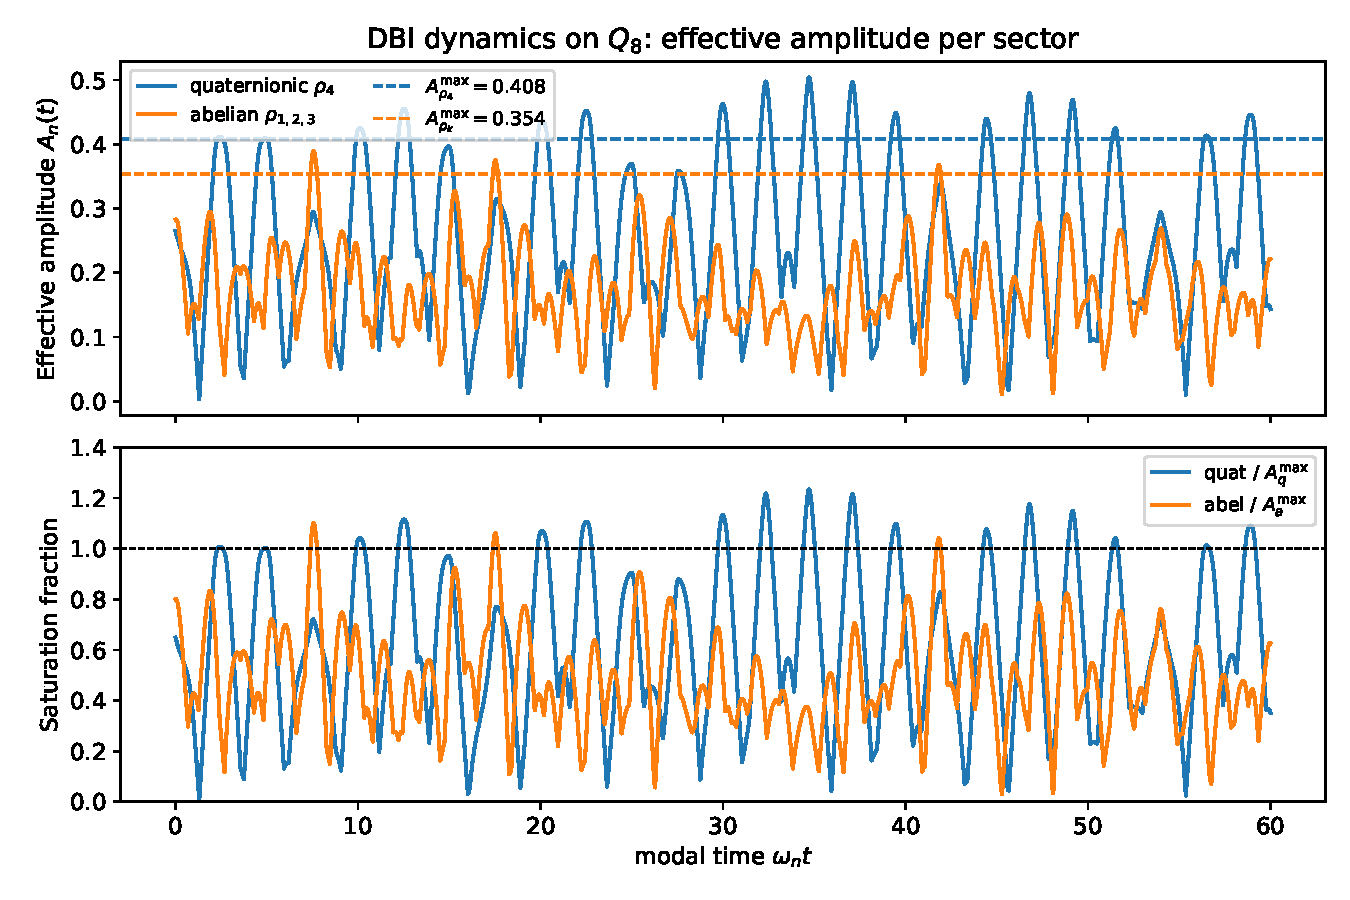
\includegraphics[width=0.9\textwidth]{fig2_Q8_DBI_dynamics}
    \caption{
      One-mode DBI dynamics on the $Q_8$ Cayley graph.
      Top: effective amplitudes in the quaternionic and abelian sectors.
      Bottom: corresponding saturation fractions relative to the exact
      admissibility bounds.
      The horizontal axis denotes the evolution parameter of the reduced
      modal dynamics.
      The quaternionic sector retains the largest admissible window,
      consistent with the spectral hierarchy derived from the bounded-flux
      constraint.
    }
    \label{fig:q8-dbi-dynamics}
  \end{figure}

  At fixed effective amplitude, the non-abelian sector thus remains less penalised
  by the weakly non-linear DBI correction, solely because $\lambda_{\rho_4}=6$
  is smaller than $\lambda_{\rho_k}=8$.
